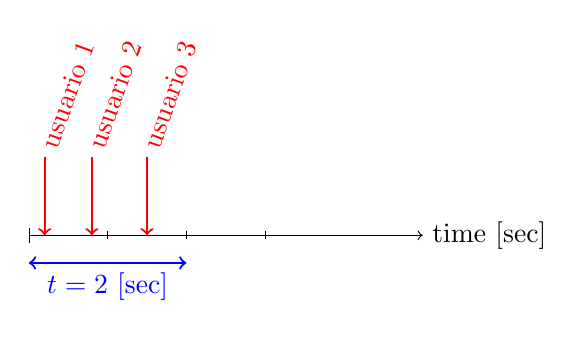
\begin{tikzpicture}
    % Time axis
    \draw[|->] (0,0) -- (5,0) node[anchor=west] {time [sec]};

    % ticks
    \draw (1,.05) -- (1,-.05);
    \draw (2,.05) -- (2,-.05);
    \draw (3,.05) -- (3,-.05);

    
    % arrivals
    \draw[->,color=red,thick] (0.2,1) node[anchor=west,rotate=70] {usuario 1} --(0.2,0);
    \draw[->,color=red,thick] (0.8,1) node[anchor=west,rotate=70] {usuario 2} --(0.8,0);
    \draw[->,color=red,thick] (1.5,1)node[anchor=west,rotate=70] {usuario 3} --(1.5,0);

    \draw[<->,color=blue,thick] (0,-.35) -- node[anchor=north,pos=0.5]{$t=2$ [sec]} (2,-.35);
\end{tikzpicture}
